\section{Prototype Implementation}
\label{sec:implementation}


This section should provide brief details of how the prototype has been implemented.
You may want to use come code snippets here, but only focus on core features and aspects.
You are not meant to copy/paste your whole application code into the report.
Focus for instance how other developers may run your application and how they might develop it further...


The example below shows how you may include code. There are similar
styles for many other langages - in case you do not use Java in your
project. You can wrap the listing into a figure in case you need to
refer to it. How to create a figure was shown in Section~\ref{sec:technology}.

\lstinputlisting[language=java]{code/BoksVolum.java}


\subsection{Backend}

We will now look into how the Kotlin code is organized. We use Kotlin with Spring Boot as the backend. The code is organized into three main services: EventService, PollService, and UserService. 
 
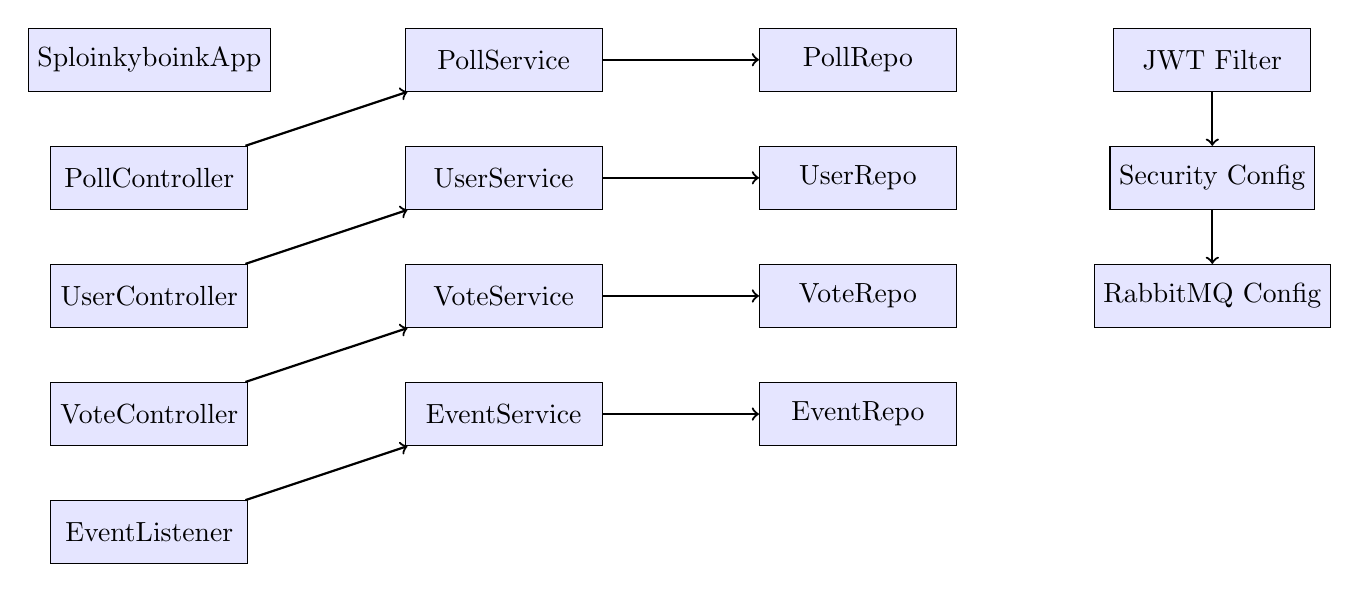
\begin{tikzpicture}[node distance=1.5cm]

% Define UML class styles
\tikzstyle{class} = [rectangle, draw=black, fill=blue!10, text centered, minimum height=0.8cm, minimum width=2.5cm]
\tikzstyle{arrow} = [->, thick, draw=black]

% Define nodes (classes)
\node[class] (sploinkyboinkApplication) {SploinkyboinkApp};
\node[class, below of=sploinkyboinkApplication] (pollController) {PollController};
\node[class, below of=pollController] (userController) {UserController};
\node[class, below of=userController] (voteController) {VoteController};
\node[class, below of=voteController] (eventListener) {EventListener};

% Define second layer nodes (Services)
\node[class, right of=sploinkyboinkApplication, xshift=3cm] (pollService) {PollService};
\node[class, below of=pollService] (userService) {UserService};
\node[class, below of=userService] (voteService) {VoteService};
\node[class, below of=voteService] (eventService) {EventService};

% Define third layer nodes (Repositories)
\node[class, right of=pollService, xshift=3cm] (pollRepository) {PollRepo};
\node[class, below of=pollRepository] (userRepository) {UserRepo};
\node[class, below of=userRepository] (voteRepository) {VoteRepo};
\node[class, below of=voteRepository] (eventRepository) {EventRepo};

% Define fourth layer nodes (Security)
\node[class, right of=pollRepository, xshift=3cm] (jwtAuthFilter) {JWT Filter};
\node[class, below of=jwtAuthFilter] (securityConfig) {Security Config};

% Define fifth layer nodes (Configurations)
\node[class, below of=securityConfig] (rabbitMQConfig) {RabbitMQ Config};

% Relationships (arrows)
\draw[arrow] (pollController) -- (pollService);
\draw[arrow] (userController) -- (userService);
\draw[arrow] (voteController) -- (voteService);
\draw[arrow] (eventListener) -- (eventService);

\draw[arrow] (pollService) -- (pollRepository);
\draw[arrow] (userService) -- (userRepository);
\draw[arrow] (voteService) -- (voteRepository);
\draw[arrow] (eventService) -- (eventRepository);

\draw[arrow] (jwtAuthFilter) -- (securityConfig);
\draw[arrow] (securityConfig) -- (rabbitMQConfig);

\end{tikzpicture}

\vspace{1cm}

The backend consists of several components, organized into layers for efficient interaction and separation of concerns. Here's a breakdown of the system’s components:

- **SploinkyboinkApp:** The main application class, acting as the entry point for the application.
- **Controllers (PollController, UserController, VoteController, EventListener):** These classes handle HTTP requests related to polls, users, votes, and events respectively. They receive inputs from the client-side and pass them to the relevant service layers.
- **Services (PollService, UserService, VoteService, EventService):** These are business logic layers that process requests from controllers. Each service is dedicated to a particular domain:
  - **PollService** manages the lifecycle of polls, including creation, updates, deletions, and voting. It also ensures users can vote only once per poll and handles results calculation.
  - **UserService** handles user registration, authentication, and CRUD operations on user data.
  - **EventService** manages logging of key events like poll creation, editing, and voting actions. These events are logged to the database and queued to RabbitMQ for further processing in an event-driven architecture.
- **Repositories (PollRepo, UserRepo, VoteRepo, EventRepo):** These components interact with the database, providing a persistent layer for the application’s data.
- **Security (JWT Filter, Security Config):** Security components that handle JWT-based authentication and configure the application’s security settings to ensure secure access.
- **RabbitMQ Config:** Configures RabbitMQ to facilitate asynchronous message processing between services, supporting scalability and decoupling.

The backend is structured to allow easy development and extension. Developers can add new features by extending the service layers and defining new event types in the EventService. The interaction between services is designed to be straightforward, with each service responsible for its specific functionality. Additionally, RabbitMQ enables scalable communication between components, ensuring that events like votes or poll updates are efficiently processed.

By using a modular structure, other developers can easily integrate new services or modify existing functionality without disturbing the overall architecture. The use of Spring Boot’s dependency injection ensures that the different layers of the application work cohesively, while the security configuration maintains the integrity of user data and access control.


